\documentclass[dvipdfmx]{jarticle}
\pagestyle{empty}
\usepackage{tikz}
\usetikzlibrary{calc,shapes,arrows.meta}
\usepackage{tabularx}
\begin{document}
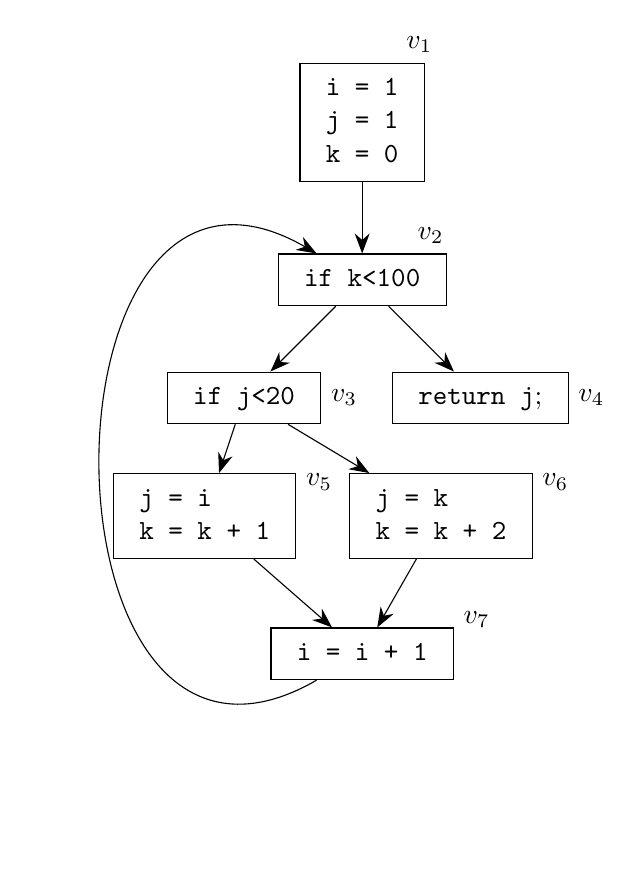
\begin{tikzpicture}
\node[draw,label={60:{$v_1$}}] (V1) at (0,0) {\begin{tabular}{l}
    \verb|i = 1|\\
    \verb|j = 1|\\
    \verb|k = 0|
\end{tabular}};
\node[draw,label={30:{$v_2$}}] (V2) at (0,-2) {\begin{tabular}{l}
    \verb|if k<100|
\end{tabular}};
\node[draw,label={0:{$v_3$}}] (V3) at (-1.5,-3.5) {\begin{tabular}{l}
    \verb|if j<20|
\end{tabular}};
\node[draw,label={0:{$v_4$}}] (V4) at (1.5,-3.5) {\begin{tabular}{l}
    \verb|return j|;
\end{tabular}};
\node[draw,label={10:{$v_5$}}] (V5) at (-2,-5) {\begin{tabular}{l}
    \verb|j = i|\\
    \verb|k = k + 1|
\end{tabular}};
\node[draw,label={10:{$v_6$}}] (V6) at (1,-5) {\begin{tabular}{l}
    \verb|j = k|\\
    \verb|k = k + 2|
\end{tabular}};
\node[draw,label={10:{$v_7$}}] (V7) at (0,-6.75) {\begin{tabular}{l}
    \verb|i = i + 1|
\end{tabular}};

\path[-{Stealth[scale=1.5]}] (V1) edge (V2) (V2) edge (V3) (V2) edge (V4);
\path[-{Stealth[scale=1.5]}] (V3) edge (V5) (V3) edge (V6) (V5) edge (V7) (V6) edge (V7);
\path[-{Stealth[scale=1.5]}] (V7) [out=210,in=150,looseness=2] edge (V2);
\end{tikzpicture}
\end{document}